% HARP illustrations: what the quantities of the framework mean, drawn for HGCal.
% Build: bash illustrations/build.sh  (pdflatex + beamer + TikZ, no external figures)
\documentclass[aspectratio=169,10pt]{beamer}
\usetheme{default}
\usecolortheme{seagull}
\setbeamertemplate{navigation symbols}{}
\setbeamertemplate{footline}{\hfill\scriptsize HARP illustrations \quad \insertframenumber/\inserttotalframenumber\hspace{1em}\vspace{0.4em}}
\setbeamercolor{frametitle}{fg=black!85}
\setbeamerfont{frametitle}{series=\bfseries,size=\large}
\usepackage{tikz}
\usetikzlibrary{arrows.meta,calc,positioning,shapes.geometric,decorations.pathreplacing,backgrounds,fit}
\usepackage{amsmath}

% ---- colours (same palette as the plots) -----------------------------------
\definecolor{cee}{HTML}{D9E7F5}      % CE-E background
\definecolor{ceh}{HTML}{F5E6D3}      % CE-H background
\definecolor{best}{HTML}{0072B2}     % best trackster
\definecolor{other}{HTML}{56B4E9}    % other tracksters
\definecolor{none}{HTML}{D55E00}     % no trackster
\definecolor{sim}{HTML}{009E73}      % sim / truth
\definecolor{track}{HTML}{000000}
\definecolor{cand}{HTML}{CC79A7}
\definecolor{grey}{HTML}{999999}

% ---- a side view of HGCal: 26 CE-E + 21 CE-H layers, z to the right ---------
% #1 = x scale (cm per layer unit), used by every slide
\newcommand{\hgcal}[1][0.18]{%
  \fill[cee] (0,0) rectangle (26*#1,4);
  \fill[ceh] (26*#1,0) rectangle (47*#1,4);
  \foreach \l in {1,...,47} {\draw[grey!60,line width=0.2pt] (\l*#1-0.5*#1,0) -- (\l*#1-0.5*#1,4);}
  \draw[black!70] (0,0) rectangle (47*#1,4);
  \node[below,font=\scriptsize] at (13*#1,0) {CE-E (layers 1--26, Si)};
  \node[below,font=\scriptsize] at (36.5*#1,0) {CE-H (layers 27--47, Si + scintillator)};
  \node[left,font=\scriptsize] at (0,2) {beam $\rightarrow$};
}
% layer cluster: a dot at (layer, y) with size ~ energy
\newcommand{\lc}[4]{\fill[#4] (#1*0.18-0.09,#2) circle (#3);}

\begin{document}

% ============================================================================
\begin{frame}{HARP: what we look at in HGCal}
\begin{columns}
\column{0.62\textwidth}
\resizebox{\linewidth}{!}{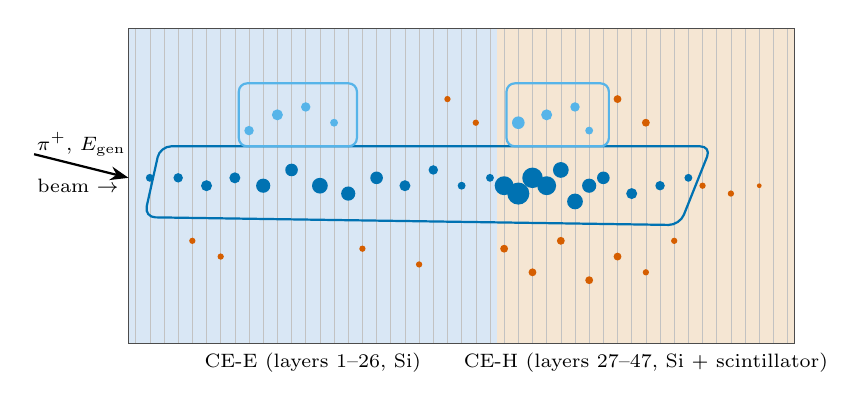
\begin{tikzpicture}[scale=1]
  \hgcal
  % hadron track entering
  \draw[track,thick,-{Stealth}] (-1.2,2.4) -- (0,2.1) node[midway,above,font=\scriptsize] {$\pi^+$, $E_{\rm gen}$};
  % shower: layer clusters
  \foreach \l/\y/\r in {2/2.1/0.05,4/2.1/0.06,6/2.0/0.07,8/2.1/0.07,10/2.0/0.09,12/2.2/0.08,14/2.0/0.1,16/1.9/0.09,18/2.1/0.08,20/2.0/0.07,22/2.2/0.06,24/2.0/0.05,26/2.1/0.05}
    {\lc{\l}{\y}{\r}{best}}
  \foreach \l/\y/\r in {27/2.0/0.12,28/1.9/0.14,29/2.1/0.13,30/2.0/0.12,31/2.2/0.1,32/1.8/0.1,33/2.0/0.09,34/2.1/0.08,36/1.9/0.07,38/2.0/0.06,40/2.1/0.05}
    {\lc{\l}{\y}{\r}{best}}
  \foreach \l/\y/\r in {9/2.7/0.06,11/2.9/0.07,13/3.0/0.06,15/2.8/0.05,28/2.8/0.08,30/2.9/0.07,32/3.0/0.06,33/2.7/0.05}
    {\lc{\l}{\y}{\r}{other}}
  \foreach \l/\y/\r in {5/1.3/0.04,7/1.1/0.04,17/1.2/0.04,21/1.0/0.04,27/1.2/0.05,29/0.9/0.05,31/1.3/0.05,33/0.8/0.05,35/1.1/0.05,37/2.8/0.05,39/1.3/0.04,41/2.0/0.04,43/1.9/0.04,45/2.0/0.03,25/2.8/0.04,23/3.1/0.04,35/3.1/0.05,37/0.9/0.04}
    {\lc{\l}{\y}{\r}{none}}
  % hulls
  \draw[best,thick,rounded corners=4pt] (0.2,1.6) -- (7.0,1.5) -- (7.4,2.5) -- (0.4,2.5) -- cycle;
  \draw[other,thick,rounded corners=3pt] (1.4,2.5) -- (2.9,2.5) -- (2.9,3.3) -- (1.4,3.3) -- cycle;
  \draw[other,thick,rounded corners=3pt] (4.8,2.5) -- (6.1,2.5) -- (6.1,3.3) -- (4.8,3.3) -- cycle;
\end{tikzpicture}}
\column{0.38\textwidth}
\footnotesize
\begin{itemize}\setlength\itemsep{4pt}
  \item \textbf{layer clusters} (dots): CLUE clusters of rec-hits on one layer; size $\propto$ energy
  \item \textcolor{best}{\textbf{best trackster}}: the CLUE3D trackster best matched to the hadron
  \item \textcolor{other}{\textbf{other tracksters}}: further tracksters sharing the hadron's hits (fragments)
  \item \textcolor{none}{\textbf{no trackster}}: layer clusters that CLUE3D did not attach to any trackster
  \item everything is measured versus $E_{\rm gen}$, per hadron type ($\pi^0,\pi^\pm,K^\pm,p,\bar p$)
\end{itemize}
\end{columns}
\end{frame}

% ============================================================================
\begin{frame}{The matching chain: gen $\rightarrow$ sim $\rightarrow$ reco $\rightarrow$ candidate}
\centering
\resizebox{\linewidth}{!}{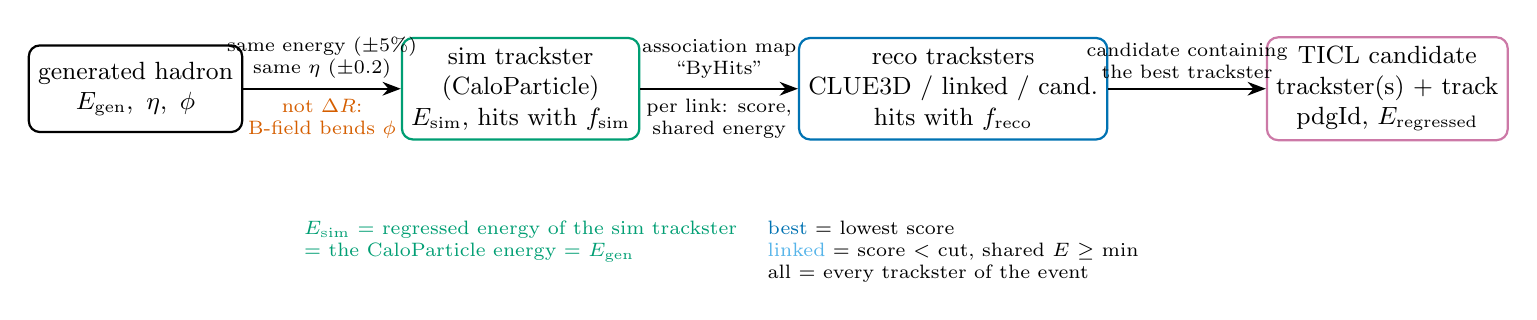
\begin{tikzpicture}[node distance=1.1cm and 2.0cm, every node/.style={font=\small},
  box/.style={draw,rounded corners,minimum height=1.1cm,minimum width=2.4cm,align=center,line width=0.8pt}]
  \node[box,draw=track] (gen) {generated hadron\\$E_{\rm gen},\ \eta,\ \phi$};
  \node[box,draw=sim,right=of gen] (sim) {sim trackster\\(CaloParticle)\\$E_{\rm sim}$, hits with $f_{\rm sim}$};
  \node[box,draw=best,right=of sim] (reco) {reco tracksters\\CLUE3D / linked / cand.\\hits with $f_{\rm reco}$};
  \node[box,draw=cand,right=of reco] (cand) {TICL candidate\\trackster(s) + track\\pdgId, $E_{\rm regressed}$};
  \draw[-{Stealth},thick] (gen) -- node[above,align=center,font=\scriptsize] {same energy ($\pm5\%$)\\same $\eta$ ($\pm0.2$)} node[below,align=center,font=\scriptsize,text=none] {not $\Delta R$:\\B-field bends $\phi$} (sim);
  \draw[-{Stealth},thick] (sim) -- node[above,align=center,font=\scriptsize] {association map\\``ByHits''} node[below,align=center,font=\scriptsize] {per link: score,\\shared energy} (reco);
  \draw[-{Stealth},thick] (reco) -- node[above,align=center,font=\scriptsize] {candidate containing\\the best trackster} (cand);
  \node[below=0.9cm of sim,align=left,font=\scriptsize,text=sim] {$E_{\rm sim}$ = regressed energy of the sim trackster\\= the CaloParticle energy = $E_{\rm gen}$};
  \node[below=0.9cm of reco,align=left,font=\scriptsize] {\textcolor{best}{best} = lowest score\\\textcolor{other}{linked} = score $<$ cut, shared $E$ $\geq$ min\\all = every trackster of the event};
\end{tikzpicture}}

\vspace{3mm}
\footnotesize The \texttt{HadronTruthMatcher} fills one \texttt{HadronMatch} per generated hadron with all of these; every analyzer reads it.
\end{frame}

% ============================================================================
\begin{frame}{The association score: hit bookkeeping, not a probability}
\begin{columns}
\column{0.5\textwidth}
\centering
\resizebox{\linewidth}{!}{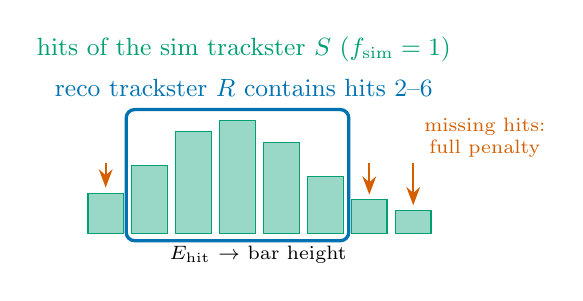
\begin{tikzpicture}[scale=0.9]
  % hits of the sim trackster S: row of squares with energies; reco trackster R covers a subset
  \node[font=\small,text=sim] at (2.2,2.6) {hits of the sim trackster $S$ ($f_{\rm sim}=1$)};
  \foreach \i/\e in {0/0.35,1/0.6,2/0.9,3/1.0,4/0.8,5/0.5,6/0.3,7/0.2} {
    \fill[sim!40] (\i*0.62,0) rectangle ++(0.5,\e*1.6);
    \draw[sim] (\i*0.62,0) rectangle ++(0.5,\e*1.6);
  }
  \node[font=\scriptsize] at (2.4,-0.3) {$E_{\rm hit}$ $\rightarrow$ bar height};
  % R covers hits 1..5
  \draw[best,very thick,rounded corners=3pt] (0.62-0.08,-0.1) rectangle (5*0.62+0.5+0.08,1.75);
  \node[font=\small,text=best] at (2.2,2.05) {reco trackster $R$ contains hits 2--6};
  \draw[none,thick,-{Stealth}] (0.25,1.0) -- (0.25,0.65);
  \draw[none,thick,-{Stealth}] (6*0.62+0.25,1.0) -- (6*0.62+0.25,0.55);
  \draw[none,thick,-{Stealth}] (7*0.62+0.25,1.0) -- (7*0.62+0.25,0.4);
  \node[font=\scriptsize,text=none,align=center] at (5.6,1.35) {missing hits:\\full penalty};
\end{tikzpicture}}
\column{0.5\textwidth}
\footnotesize
\[
  \mathrm{score}(S\!\to\!R)=\frac{\sum_{\rm hits}(f_{\rm sim}-f_{\rm reco})^2E_{\rm hit}^2}{\sum_{\rm hits}f_{\rm sim}^2E_{\rm hit}^2}
\]
\begin{itemize}\setlength\itemsep{3pt}
  \item $f$: fraction of the hit's energy assigned to the object
  \item hit in $S$ but not in $R$: penalty $E_{\rm hit}^2$; hit in both: no penalty
  \item bounded: 0 = $R$ contains all of $S$, 1 = nothing shared
  \item for all-or-nothing hits: \textbf{score $\approx 1-$ ($E^2$-weighted fraction of $S$ captured by $R$)}
  \item $E^2$ weighting: dominated by the few highest-energy hits
  \item reco$\to$sim score: same formula normalised to $R$'s hits
\end{itemize}
\scriptsize Computed in CMSSW from the simulated hit fractions (\texttt{AllTracksterToSimTracksterAssociatorsByHitsProducer}); deterministic, no training.
\end{columns}
\end{frame}

% ============================================================================
\begin{frame}{Best, linked, all: the reco energy definitions}
\begin{columns}
\column{0.55\textwidth}
\resizebox{\linewidth}{!}{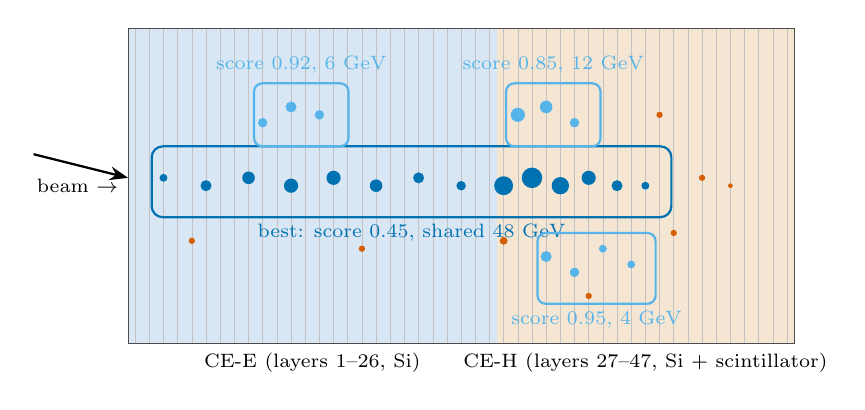
\begin{tikzpicture}[scale=1]
  \hgcal
  \draw[track,thick,-{Stealth}] (-1.2,2.4) -- (0,2.1);
  \foreach \l/\y/\r in {3/2.1/0.05,6/2.0/0.07,9/2.1/0.08,12/2.0/0.09,15/2.1/0.09,18/2.0/0.08,21/2.1/0.07,24/2.0/0.06,27/2.0/0.12,29/2.1/0.13,31/2.0/0.11,33/2.1/0.09,35/2.0/0.07,37/2.0/0.05}
    {\lc{\l}{\y}{\r}{best}}
  \foreach \l/\y/\r in {10/2.8/0.06,12/3.0/0.07,14/2.9/0.06,28/2.9/0.09,30/3.0/0.08,32/2.8/0.06}
    {\lc{\l}{\y}{\r}{other}}
  \foreach \l/\y/\r in {30/1.1/0.07,32/0.9/0.06,34/1.2/0.05,36/1.0/0.05}
    {\lc{\l}{\y}{\r}{other}}
  \foreach \l/\y/\r in {5/1.3/0.04,17/1.2/0.04,27/1.3/0.05,33/0.6/0.04,39/1.4/0.04,41/2.1/0.04,43/2.0/0.03,38/2.9/0.04}
    {\lc{\l}{\y}{\r}{none}}
  \draw[best,thick,rounded corners=4pt] (0.3,1.6) -- (6.9,1.6) -- (6.9,2.5) -- (0.3,2.5) -- cycle;
  \node[best,font=\scriptsize] at (3.6,1.4) {best: score 0.45, shared 48 GeV};
  \draw[other,thick,rounded corners=3pt] (1.6,2.5) -- (2.8,2.5) -- (2.8,3.3) -- (1.6,3.3) -- cycle;
  \node[other,font=\scriptsize,above] at (2.2,3.3) {score 0.92, 6 GeV};
  \draw[other,thick,rounded corners=3pt] (4.8,2.5) -- (6.0,2.5) -- (6.0,3.3) -- (4.8,3.3) -- cycle;
  \node[other,font=\scriptsize,above] at (5.4,3.3) {score 0.85, 12 GeV};
  \draw[other,thick,rounded corners=3pt] (5.2,0.5) -- (6.7,0.5) -- (6.7,1.4) -- (5.2,1.4) -- cycle;
  \node[other,font=\scriptsize] at (5.95,0.3) {score 0.95, 4 GeV};
\end{tikzpicture}}
\column{0.45\textwidth}
\footnotesize
Response $R = E_{\rm reco}/E_{\rm gen}$ with $E_{\rm reco}$ one of:
\begin{itemize}\setlength\itemsep{3pt}
  \item \textcolor{best}{\textbf{bestRaw}}: raw energy of the lowest-score trackster
  \item \textcolor{other}{\textbf{linkedRaw}}: sum over all tracksters sharing hits (score $<$ \texttt{linkScoreCut}, default 1)
  \item \textbf{allRaw}: every trackster of the event (= linked for a gun, differs with pile-up)
  \item \textcolor{sim}{\textbf{simRaw}}: the sim trackster, i.e.\ what the hadron deposited
  \item \textcolor{none}{\textbf{layerClusters}}: all layer clusters, clustered or not
  \item \textcolor{cand}{\textbf{candidate}}: TICL candidate (regressed); \textbf{candidateRaw}: its raw sum
\end{itemize}
``raw'' = sum of layer-cluster energies, no calibration. The plots show scale $\langle R\rangle$ and resolution $\sigma(R)/\langle R\rangle$ vs $E_{\rm gen}$ from Gaussian fits in each $E_{\rm gen}$ bin.
\end{columns}
\end{frame}

% ============================================================================
\begin{frame}{Where the energy goes: the energy budget}
\begin{columns}
\column{0.5\textwidth}
\centering
\resizebox{\linewidth}{!}{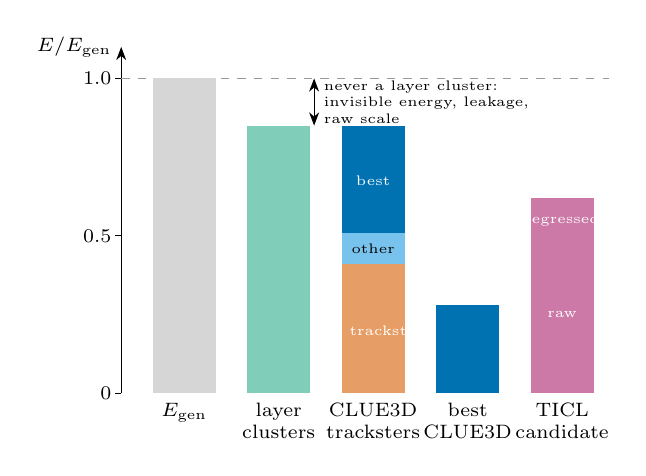
\begin{tikzpicture}[scale=1]
  % waterfall for pi+ at 85 GeV (numbers from the full-sample study)
  \draw[-{Stealth}] (0,0) -- (0,4.4) node[left,font=\scriptsize] {$E/E_{\rm gen}$};
  \foreach \y in {0,0.5,1.0} {\draw (-0.08,\y*4) -- (0,\y*4) node[left,font=\scriptsize] {\y};}
  \draw[dashed,grey] (0,4) -- (6.2,4);
  % bars
  \fill[grey!40] (0.4,0) rectangle (1.2,4);    \node[font=\scriptsize,below] at (0.8,0) {$E_{\rm gen}$};
  \fill[sim!50] (1.6,0) rectangle (2.4,3.4);   \node[font=\scriptsize,below,align=center] at (2.0,0) {layer\\clusters};
  \fill[none!60] (2.8,0) rectangle (3.6,1.64); \fill[other!80] (2.8,1.64) rectangle (3.6,2.04); \fill[best] (2.8,2.04) rectangle (3.6,3.4);
  \node[font=\scriptsize,below,align=center] at (3.2,0) {CLUE3D\\tracksters};
  \fill[best] (4.0,0) rectangle (4.8,1.12);    \node[font=\scriptsize,below,align=center] at (4.4,0) {best\\CLUE3D};
  \fill[cand!60] (5.2,0) rectangle (6.0,1.84); \fill[cand] (5.2,0) rectangle (6.0,2.48);
  \node[font=\scriptsize,below,align=center] at (5.6,0) {TICL\\candidate};
  % annotations
  \draw[{Stealth}-{Stealth},thin] (2.45,3.4) -- (2.45,4) node[midway,right,font=\tiny,align=left] {never a layer cluster:\\invisible energy, leakage,\\raw scale};
  \node[font=\tiny,text=white] at (3.2,0.8) {no trackster};
  \node[font=\tiny,text=white] at (3.2,2.7) {best};
  \node[font=\tiny] at (3.2,1.84) {other};
  \node[font=\tiny,text=white,align=center] at (5.6,2.2) {regressed};
  \node[font=\tiny,text=white] at (5.6,1.0) {raw};
\end{tikzpicture}}
\column{0.5\textwidth}
\footnotesize
\texttt{EnergyBudgetAnalyzer} classifies every layer cluster of the event:
\begin{itemize}\setlength\itemsep{3pt}
  \item in the \textcolor{best}{best trackster}, in \textcolor{other}{another trackster}, or in \textcolor{none}{no trackster} (shared clusters split $1/n$);
  \item as fractions of the layer-cluster energy (stack to 1) or divided by $E_{\rm gen}$ (stack to the layer-cluster response);
  \item split by compartment (CE-E / CE-H), per layer in $E_{\rm gen}$ windows, and versus the layer-cluster energy.
\end{itemize}
\vspace{1mm}
Example $\pi^+$, 85 GeV: 0.85 reaches layer clusters, 0.51 is in tracksters, 0.28 in the best one; linking brings the candidate trackster to 0.46 raw, the regression to 0.62.
\end{columns}
\end{frame}

% ============================================================================
\begin{frame}{Efficiency, purity, duplicate, fake (CMSSW HGCalValidation definitions)}
\centering
\resizebox{\linewidth}{!}{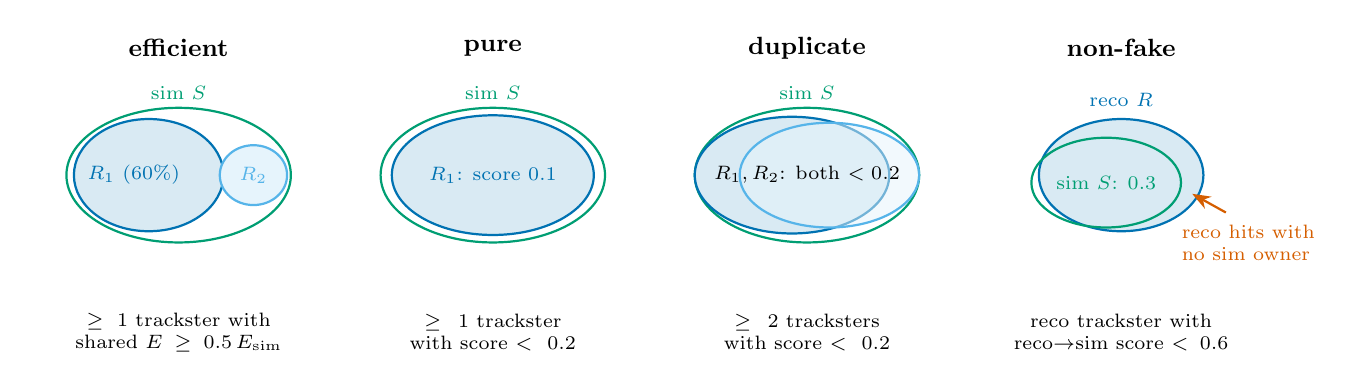
\begin{tikzpicture}[scale=0.95, every node/.style={font=\scriptsize}]
  % four panels; each: a sim trackster (green ellipse) and reco tracksters (blue ellipses) with text
  \foreach \x/\title/\txt in {0/{efficient}/{$\geq1$ trackster with shared $E \geq 0.5\,E_{\rm sim}$}, 4.2/{pure}/{$\geq1$ trackster with score $<0.2$}, 8.4/{duplicate}/{$\geq2$ tracksters with score $<0.2$}, 12.6/{non-fake}/{reco trackster with reco$\to$sim score $<0.6$}} {
    \node[font=\small\bfseries] at (\x+1.6,3.2) {\title};
    \node[align=center,text width=3.6cm] at (\x+1.6,-0.6) {\txt};
  }
  % efficient: one big reco covering > half of sim
  \draw[sim,thick] (1.6,1.5) ellipse (1.5 and 0.9); \node[sim] at (1.6,2.6) {sim $S$};
  \draw[best,thick,fill=best!15] (1.2,1.5) ellipse (1.0 and 0.75); \node[best] at (1.0,1.5) {$R_1$ (60\%)};
  \draw[other,thick,fill=other!15] (2.6,1.5) ellipse (0.45 and 0.4); \node[other] at (2.6,1.5) {$R_2$};
  % pure: one reco matches almost everything
  \draw[sim,thick] (5.8,1.5) ellipse (1.5 and 0.9); \node[sim] at (5.8,2.6) {sim $S$};
  \draw[best,thick,fill=best!15] (5.8,1.5) ellipse (1.35 and 0.8); \node[best] at (5.8,1.5) {$R_1$: score 0.1};
  % duplicate: two recos each with low score -> only possible when hits are shared
  \draw[sim,thick] (10.0,1.5) ellipse (1.5 and 0.9); \node[sim] at (10.0,2.6) {sim $S$};
  \draw[best,thick,fill=best!15] (9.8,1.5) ellipse (1.3 and 0.78); \draw[other,thick,fill=other!15,fill opacity=0.5] (10.3,1.5) ellipse (1.2 and 0.7);
  \node at (10.0,1.5) {$R_1,R_2$: both $<0.2$};
  % non-fake: reco trackster mostly inside a sim trackster
  \draw[best,thick,fill=best!15] (14.2,1.5) ellipse (1.1 and 0.75); \node[best] at (14.2,2.5) {reco $R$};
  \draw[sim,thick] (14.0,1.4) ellipse (1.0 and 0.6); \node[sim] at (14.0,1.4) {sim $S$: 0.3};
  \draw[none,thick,-{Stealth}] (15.6,1.0) -- (15.15,1.25); \node[none,align=left] at (15.9,0.6) {reco hits with\\no sim owner};
\end{tikzpicture}}

\vspace{1mm}
\resizebox{0.95\textwidth}{!}{\begin{tabular}{llll}
quantity & per & CMSSW parameter (default) & HARP plot \\\hline
efficiency & sim trackster & \texttt{minTSTSharedEneFracEfficiency} (0.5) & \texttt{matching/efficient/vsE} \\
purity, duplicate & sim trackster & \texttt{maxSimToRecoScoreForPurity/Duplicate} (0.2) & \texttt{matching/pure, duplicate/vsE} \\
non-fake & reco trackster & \texttt{maxRecoToSimScoreForNonFake} (0.6) & \texttt{matching/nonFake/vsE, vsRawE} \\
\end{tabular}}

\vspace{1mm}\scriptsize Purity asks for \emph{one} trackster containing $\sim80\%$ of the hadron's $E^2$-weighted hits: a hadron shower split into several good tracksters fails it. HARP adds \texttt{hasReco} (any link at all) as the lower bar.
\end{frame}

% ============================================================================
\begin{frame}{Shower variables for identification (per trackster)}
\begin{columns}
\column{0.58\textwidth}
\resizebox{\linewidth}{!}{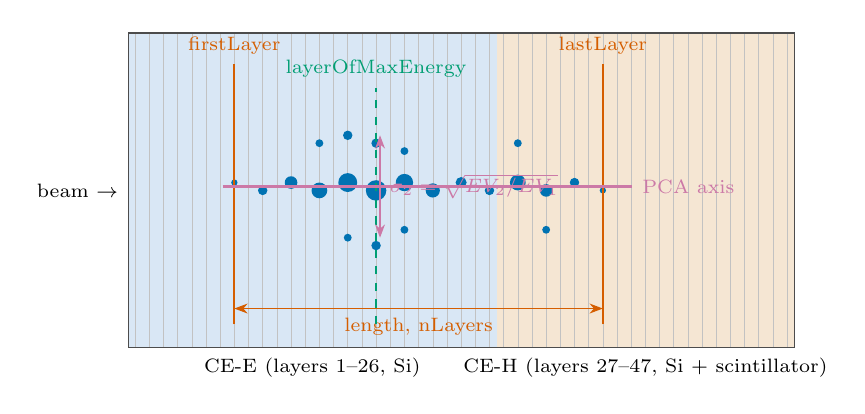
\begin{tikzpicture}[scale=1]
  \hgcal
  \foreach \l/\y/\r in {8/2.1/0.04,10/2.0/0.06,12/2.1/0.08,14/2.0/0.1,16/2.1/0.12,18/2.0/0.13,20/2.1/0.11,22/2.0/0.09,24/2.1/0.07,26/2.0/0.06,28/2.1/0.1,30/2.0/0.08,32/2.1/0.06,34/2.0/0.04}
    {\lc{\l}{\y}{\r}{best}}
  \foreach \l/\y/\r in {14/2.6/0.05,16/2.7/0.06,18/2.6/0.06,20/2.5/0.05,16/1.4/0.05,18/1.3/0.06,20/1.5/0.05,28/2.6/0.05,30/1.5/0.05}
    {\lc{\l}{\y}{\r}{best}}
  % first / last layer
  \draw[none,thick] (8*0.18-0.09,0.3) -- (8*0.18-0.09,3.6) node[above,font=\scriptsize,text=none] {firstLayer};
  \draw[none,thick] (34*0.18-0.09,0.3) -- (34*0.18-0.09,3.6) node[above,font=\scriptsize,text=none] {lastLayer};
  \draw[{Stealth}-{Stealth},none] (8*0.18-0.09,0.5) -- (34*0.18-0.09,0.5) node[midway,below,font=\scriptsize,text=none] {length, nLayers};
  % layer of max
  \draw[sim,thick,dashed] (18*0.18-0.09,0.3) -- (18*0.18-0.09,3.3) node[above,font=\scriptsize,text=sim] {layerOfMaxEnergy};
  % PCA axis and transverse width
  \draw[cand,thick] (1.2,2.05) -- (6.4,2.05) node[right,font=\scriptsize,text=cand] {PCA axis};
  \draw[{Stealth}-{Stealth},cand] (3.2,1.4) -- (3.2,2.7) node[midway,right,font=\scriptsize,text=cand] {$\sigma_2=\sqrt{EV_2/EV_1}$};
\end{tikzpicture}}
\column{0.42\textwidth}
\footnotesize
From \texttt{ShowerVariablesProducer} (\texttt{pid/} plots, best trackster):
\begin{itemize}\setlength\itemsep{2pt}
  \item depth: \textbf{firstLayer}, \textbf{lastLayer}, \textbf{length} (cm), \textbf{nLayers}, \textbf{layerOfMaxEnergy}, \textbf{rmsLayer}
  \item compartments: \textbf{fractionEE} = $E_{\rm CE\text{-}E}/(E_{\rm CE\text{-}E}+E_{\rm CE\text{-}H})$, \textbf{emFraction} = \texttt{raw\_em\_energy/raw\_energy}
  \item shape: \textbf{sigma2}, \textbf{sigma3} from the PCA eigenvalues, \textbf{maxLayerEnergyFraction}, \textbf{nLayerClusters}
  \item plus the TICL \textbf{candidate pdgId} versus $E_{\rm gen}$ (the identification TICL already makes)
\end{itemize}
$\pi^0$: compact, all in CE-E, $\sim$25 layers. Charged hadrons: start anywhere, reach CE-H, wide spread of nLayers.
\end{columns}
\end{frame}

\end{document}
